\documentclass[5p,twocolumn,times,number]{elsarticle}

\usepackage{caption}
%\captionsetup[figure]{font=scriptsize}
\captionsetup[figure]{font=footnotesize}

\usepackage{bbding}
\usepackage{pifont}
\usepackage{graphicx}
\usepackage{amsmath}  
\usepackage{subfig}
%\usepackage{cite}
\usepackage{amsmath}
\usepackage{cleveref}
\usepackage{textcomp}
\usepackage{tabularx}
\usepackage{booktabs} 
\usepackage{multirow}
%\usepackage{gensymb}
\usepackage{hepunits} 
%%
%% This simulates the banner introduced in NIMA after post-processing.
\def\pmbanner{{\hrule height 1 pt}\vskip35pt{NIMA POST-PROCESS BANNER TO BE REMOVED AFTER FINAL ACCEPTANCE}\vskip35pt{\hrule height 4pt}\vskip20pt}
%% End of definition. Please insert the command \pmbanner before your contibution's title
%%
%% \title{\pmbanner Title of the contribution}
%%
% Joel wrote this (thanks!!)

\addunit{\Gray}{Gy}
\DeclareMathOperator\erf{erf}
\DeclareRobustCommand{\microns}{\;\micro\metre\;}
\DeclareRobustCommand{\microSecond}{\;\micro\second\;}
\DeclareRobustCommand{\nanoSecond}{\;\nano\second\;}
\DeclareRobustCommand{\cm}{\;\centi\metre\;}
\DeclareRobustCommand{\mm}{\;\milli\metre\;}
\DeclareRobustCommand{\nm}{\;\nano\metre\;}
\DeclareRobustCommand{\kHz}{\;\kilo\hertz\;}
\DeclareRobustCommand{\pT}{${{p}_{\mbox{\small{t}}}}$}
\DeclareRobustCommand{\cmSquared}{\;\centi\metre\rpsquared\;}
\DeclareRobustCommand{\cmSq}{\;\centi\metre\textsuperscript{2}\;}
\DeclareRobustCommand{\mmSq}{\;\milli\metre\textsuperscript{2}\;}
\DeclareRobustCommand{\MHz}{\;\mega\hertz\;}
\DeclareRobustCommand{\deg}{\;${^\circ}$\Celsius\;}
\DeclareRobustCommand{\kGy}{\;\kilo\Gray\;}
\DeclareRobustCommand{\kGyH}{\;\kilo\Gray\per\hour\;}
\DeclareRobustCommand{\mV}{\;\milli\volt\;}
\DeclareRobustCommand{\mA}{\;\milli\ampere\;}
\DeclareRobustCommand{\MVcm}{\;\mega\volt\per\centi\metre\;}
\DeclareRobustCommand{\NotMax}{N_{\mbox{\tiny{OT,max}}}}
\DeclareRobustCommand{\Not}{N_{\mbox{\tiny{OT}}}}
\DeclareRobustCommand{\Rot}{r_{\mbox{\tiny{OT}}}}
\DeclareRobustCommand{\Fot}{f_{\mbox{\tiny{OT}}}}
\DeclareRobustCommand{\dNot}{\dot N_{\mbox{\tiny{OT}}}}
\DeclareRobustCommand{\NitMax}{N_{\mbox{\tiny{SiH}}}}
\DeclareRobustCommand{\Nit}{N_{\mbox{\tiny{IT}}}}
\DeclareRobustCommand{\NitInit}{N_{\mbox{\tiny{IT,0}}}}
\DeclareRobustCommand{\NotInit}{N_{\mbox{\tiny{OT,0}}}}
\DeclareRobustCommand{\interface}{Si-SiO$_{2}$\;}
\DeclareRobustCommand{\SiO}{SiO$_{2}$\;}
\DeclareRobustCommand{\Co}{$^{60}$Co }
\DeclareRobustCommand{\eV}{\;\electronvolt\;}
\DeclareRobustCommand{\keV}{\;\kilo\electronvolt\;}
\DeclareRobustCommand{\MeV}{\;\mega\electronvolt\;}
\DeclareRobustCommand{\GeV}{\;\giga\electronvolt\;}
\DeclareRobustCommand{\TeV}{\;\tera\electronvolt\;}
\DeclareRobustCommand{\Vthr}{V_{\mbox{\tiny{thr}}}}
\DeclareRobustCommand{\Nthr}{N_{\mbox{\tiny{thr}}}}
\DeclareRobustCommand{\Neff}{N_{\mbox{\tiny{eff}}}}
\DeclareRobustCommand{\Ileak}{I_{\mbox{\tiny{leak}}}}
\DeclareRobustCommand{\IpreIrrad}{I_{\mbox{\tiny{pre-irrad}}}}
\DeclareRobustCommand{\Tthr}{t_{\mbox{\tiny{critical}}}}
\DeclareRobustCommand{\Dcritical}{d_{\mbox{\tiny{critical}}}}
\DeclareRobustCommand{\Nmax}{N_{\mbox{\tiny{max}}}}
\DeclareRobustCommand{\fb}{\;\femto\barn$^{-1}$\;}
\DeclareRobustCommand{\Vdd}{V${_{\mbox{\small{DDD}}}}$}
\DeclareRobustCommand{\Vda}{V${_{\mbox{\small{DDA}}}}$}

\setcounter{topnumber}{2}
\setcounter{bottomnumber}{2}
\setcounter{totalnumber}{4}
\renewcommand{\topfraction}{0.95}
\renewcommand{\bottomfraction}{0.85}
\renewcommand{\textfraction}{0.15}
\renewcommand{\floatpagefraction}{0.99}
\renewcommand{\textfraction}{0.1}
\setlength{\floatsep}{5pt plus 2pt minus 2pt}
\setlength{\textfloatsep}{5pt plus 2pt minus 2pt}
\setlength{\intextsep}{5pt plus 2pt minus 2pt}

%Copied from standard CMS
\newcommand{\pt}{\ensuremath{p_{\mathrm{T}}}\xspace}

\begin{document}

\begin{frontmatter}

%% Note: \pmbanner before the actual title
\title{\pmbanner Recent developments in the CBC3, a CMS micro-strip readout ASIC for track-trigger modules at the HL-LHC}
%%

\author[add1,add2]{F.~Author1\corref{cor}}
%\ead{f.author1@earth.org}
\author[add3]{J.~Author2}
\author[add6]{M.~Author3}

%\cortext[cor]{Corresponding author}

\address[add1]{Institute 1, City, Country}
\address[add2]{Institute 2, City, Country}
\address[add3]{Institute 3, City, Country}
\address[add6]{Institute 6, City, Country}

\begin{abstract}
The CMS Binary Chip (CBC) is the front-end readout ASIC planned for the outermost layers of the CMS Phase 2 silicon outer tracker. Results from an extensive irradiation campaign carried out on the CBC3, the first version of the ASIC to include the full trigger logic circuitry, have demonstrated that the chip is capable of withstanding the levels of radiation expected at the HL-LHC, with only a slight (${<1\%}$) increase in power consumption. Results from the irradiation campaign, and details of the novel damage model developed to describe the measurements and extrapolate to the final operating conditions, will be presented. Additionally results from the Fermilab test beam facility will be shown that demonstrate the full functionality of the stub-finding logic.
% * <dr.joel.goldstein@gmail.com> 2018-07-03T11:50:38.817Z:
% 
% Removed the number "three" to avoid ambiguity with layer vs double layer
% 
% ^.
\end{abstract}

\begin{keyword}
Tracking detectors \sep Radiation Effects \sep Total Ionizing Dose  \sep ASICs 

\PACS 29.40.Cs \sep 29.40.Gx    
\end{keyword}
\end{frontmatter}

\section{Introduction}
% add citations to cms ot upgrade and lhc upgrade 
The Phase-2 CMS silicon tracker upgrade \cite{CMSouterTrackerPh2TDR} will have to provide high-quality physics data while operating at the extreme beam intensities and particle collision rates foreseen at the high-luminosity upgrade of the Large Hadron Collider (HL-LHC). The outer tracker (OT) will be built from double-layered modules, each consisting of two strip (2S), or one pixel and one strip (PS) silicon sensors.
% The 2S modules in the outermost three layers (radii greater than 600mm). 
% add reference to TDR again for the module drawing 
\begin{figure}[!htbp]
\centering
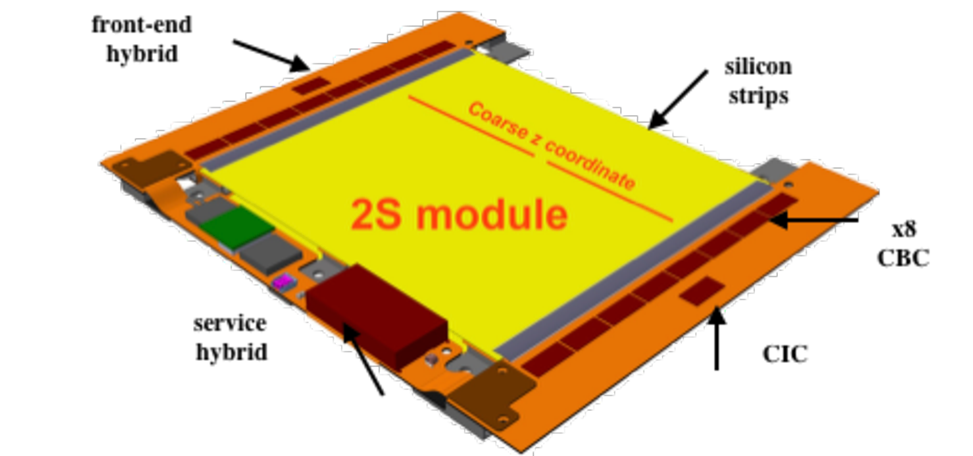
\includegraphics[width=0.75\linewidth]{Figures/Drawing_2Smodule.pdf}
\vspace*{-2mm}
\caption[2S module.]{An OT 2S module with two front-end hybrids containing sixteen CBC3s for read out the full module. A service hybrid will provide power and data connectivity.} 
\label{fig:Schematic2Smodule}
\end{figure} 

A single module can identify high transverse momentum tracks by looking for a pair of coincident hits (a stub) in nearby channels in the two closely separated sensors. Stubs from different layers can then be combined into tracks in off-detector electronics. The CMS Binary Chip (CBC) is a 254-channel front-end ASIC manufactured in 130 nm CMOS technology for the readout of the 2S modules (shown in \cref{fig:Schematic2Smodule}). The CBC3 \cite{CBC3} is the final prototype of the ASIC and the first to include the full logic circuitry required for stub finding.



% probably can live without this bit...
% % JG - stripped it down a bit, need to add reference
% % S.S - trying without this bit (! no space!! ) 
% The CBC generates a binary value for each connected strip to indicate whether the measured charge exceeded a set threshold (Vth in Figure.\cref{fig:CBC3}). The input channels are connected alternately to the strips on the two sensor layers; thus enabling the stub finding circuitry to search for correlated hits in the two layers within a programmable correlation window. 

% The location and directional data for all identified stubs, along with error and synchronization bits, are shared across five differential Scalable Low-Voltage Signaling (SLVS) pads and output from the CBC3 at a rate of $320$\MHz. 
% cite Kirika's Hiroshima paper/ M.Pedyyrech's TWEPP paper 
% \begin{figure}[htbp]
% \centering
% 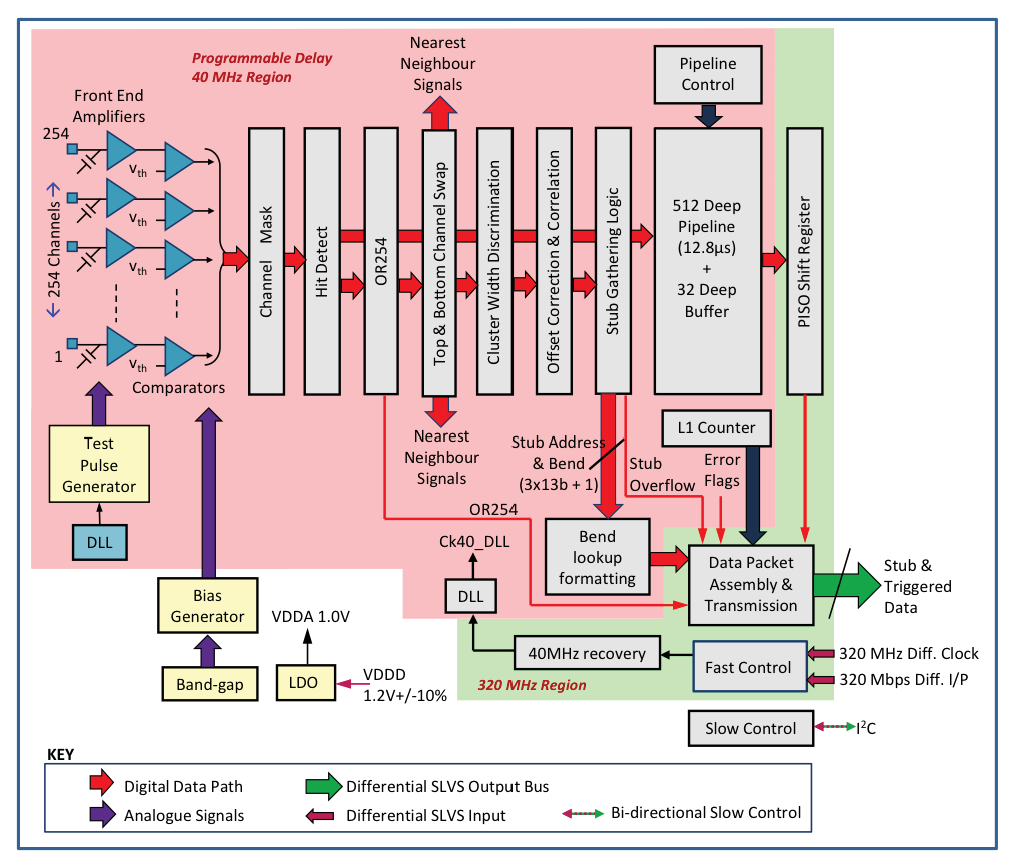
\includegraphics[width=0.9\linewidth]{Figures/Architecture_CBC3.eps}
%  \caption[Architecture of CBC3.]{A simplified block diagram describing the architecture of the CBC3: data from up to a maximum of 512 bunch crossings can be stored on-chip to allow time for the L1 trigger system to decide which event data should be read out for further processing.}
%  \label{fig:Architecture_CBC3}
% \end{figure} 

% Drop these figures if you're running out of space
\begin{figure}[!htbp]
\centering
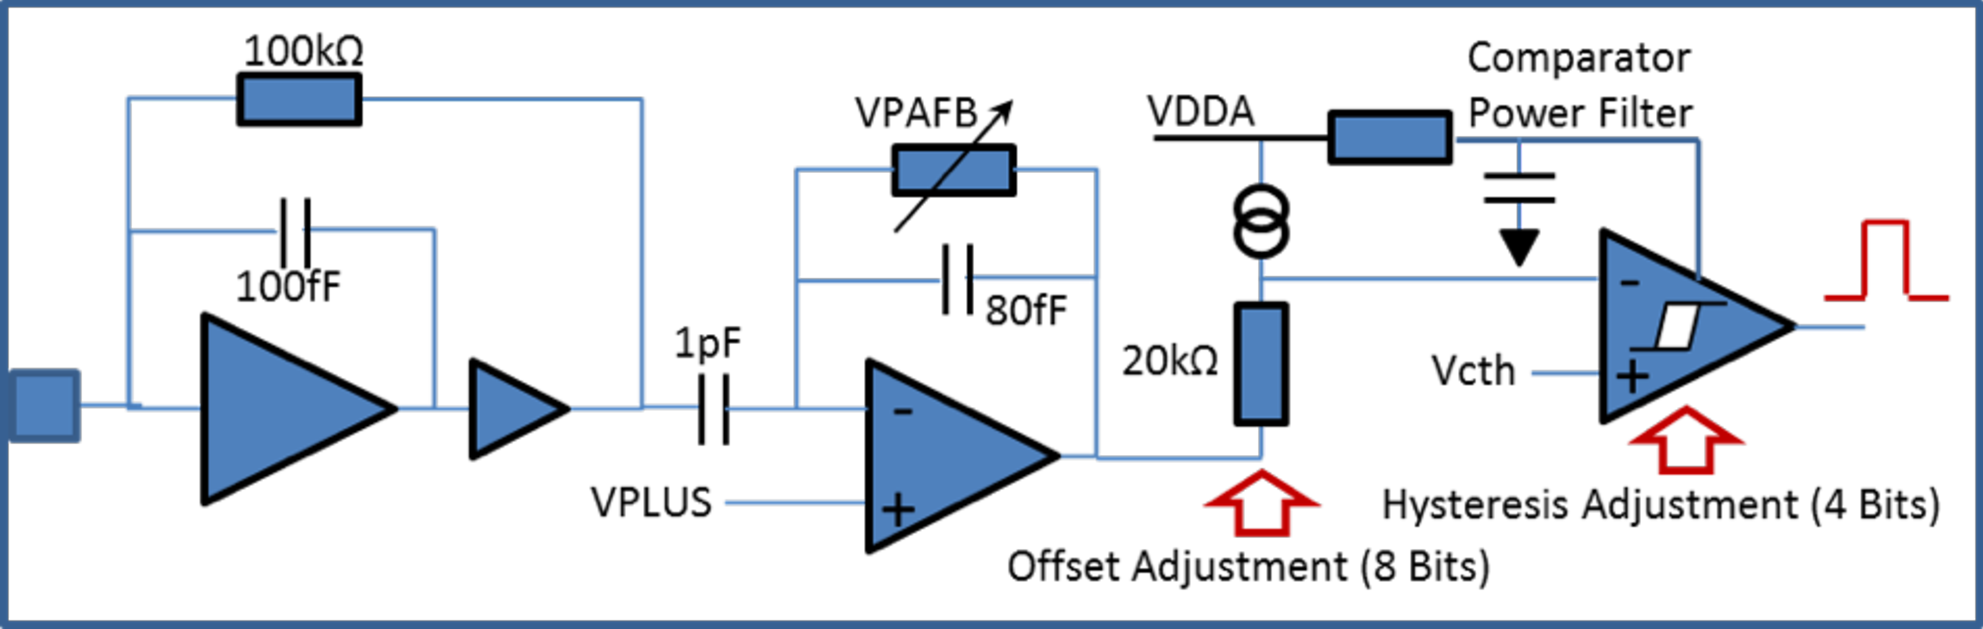
\includegraphics[width=0.9\linewidth]{Figures/Architecture_AnalogueFE}
\vspace*{-2mm}
\caption[Fit.]{A schematic of the CBC3 analogue front-end.}
\label{fig:Architecture_AnalogueFE}
\end{figure} 
% \begin{figure}[!htbp]
% \centering
% 	\subfloat[][The architecture of the CBC3.]
%   {
%     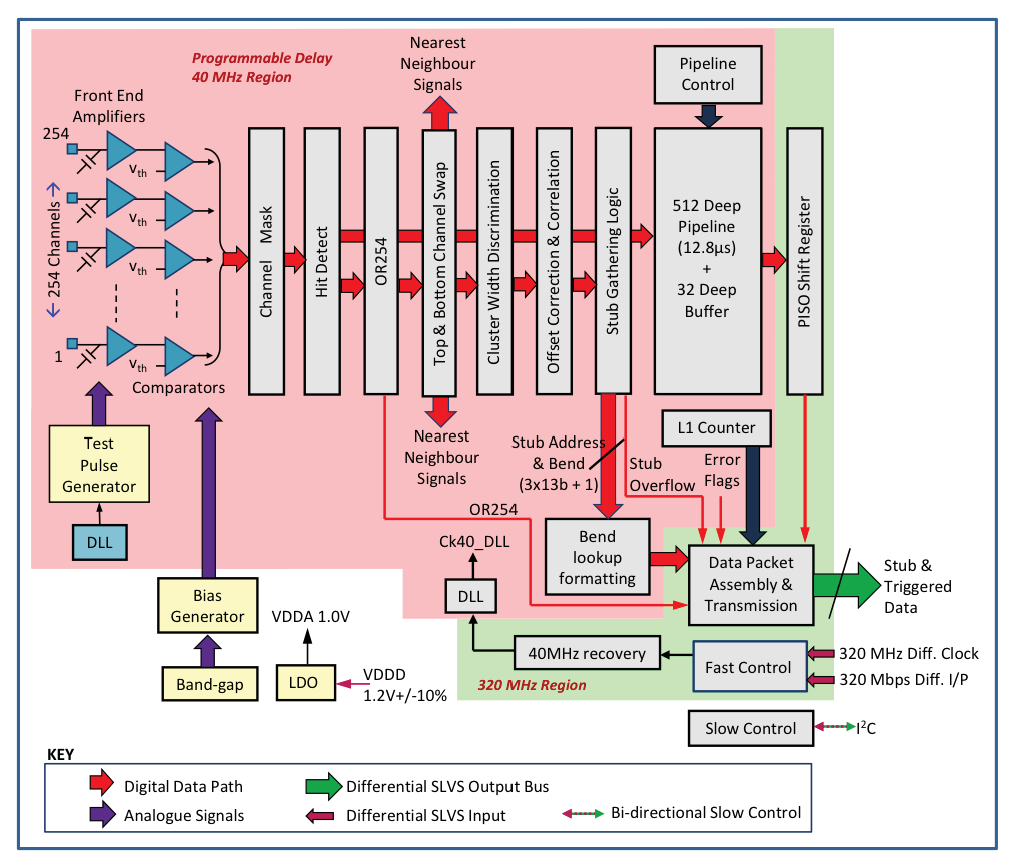
\includegraphics[width=0.9\linewidth]{Figures/Architecture_CBC3.eps}
%     \label{fig:Architecture_CBC3}
%   }
%   \quad
%   \subfloat[][Schematic of the CBC3's analogue front-end.]
%   {
%     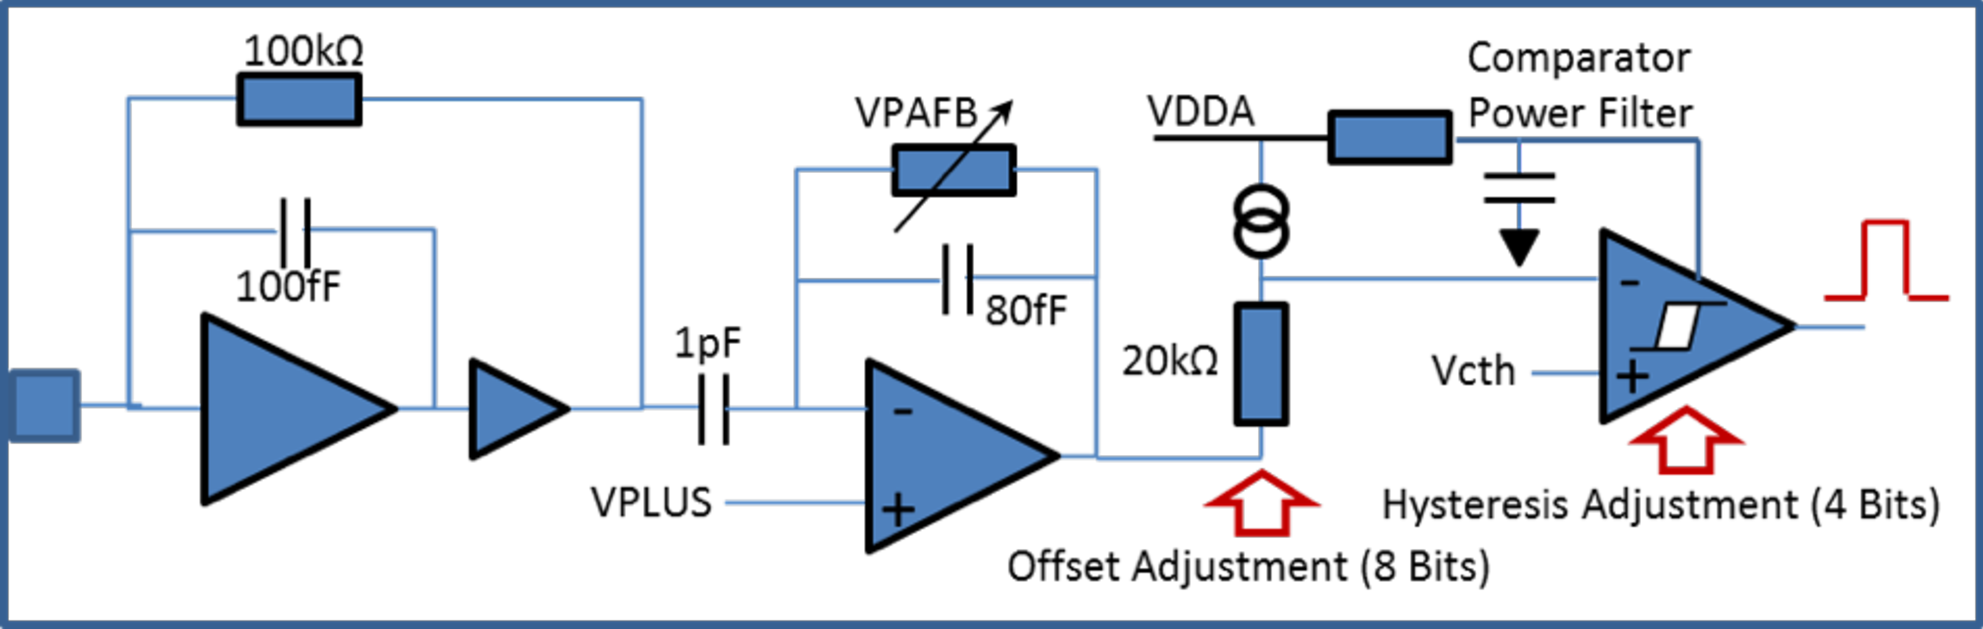
\includegraphics[width=0.9\linewidth]{Figures/Architecture_AnalogueFE}
%     \label{fig:Architecture_AnalogueFE}
%   }
%   \caption[Fit.]{Simplified block diagrams describing the architecture of the CBC3 and its analogue front-end.}
%   \label{fig:CBC3}
% \end{figure} 
 
%reference to CBC2 radiation testing (BragaThesis)
Total ionizing dose (TID) tests performed on the previous prototype \cite{CBC2nim} of the CBC showed a large, but temporary, increase in digital current and a pipeline sensitivity to occupancy. Both effects were attributed to radiation-induced leakage in the SRAM elements of the pipeline which motivated the decision to modify the SRAM block in the CBC3. 
% The NMOS read- and write-access transistors in the SRAM block were replaced with more radiation-resistant PMOS devices, and the NMOS pull-down transistors of the SRAM cross-coupled inverters were replaced with more radiation-resistant enclosed layout (ELT) NMOS devices. 

In this report the results of an X-ray irradiation campaign measuring the radiation-tolerance of the CBC3 are reported. A radiation damage model, developed to extrapolate the results to HL-LHC operating conditions, will also be described.
\section{Experimental Procedure}
\label{sec:ExpProc}
Nine CBC3 chips were irradiated, using the CERN Seifert RP149 X-ray machine, at a variety of dose rates (${0.11\pm0.02}$\kGyH to ${23.0\pm4.6}$\kGyH) and temperatures (${-20}$\deg to ${5}$\deg). The temperature of the chips were controlled and monitored throughout the irradiation, and the dose rates were measured, with an uncertainty of ${20}$\%, using a calibrated PIN diode. 
%machine's high-power cooling system was used to control the temperature of the chips, monitored using a thermocouple placed close to the chip, during irradiation. 
%connected to a source-measure unit with a high-precision ammeter.
%and its dry-air injection system was used to prevent condensation.
% Is the temperature statement true or necessary? The dew point in Geneva is often close to 20C.
% S.S changed 
%A thermocouple, placed close to the chip, was used to measure the temperature inside the X-ray chamber. 
% S.S - removed the table and added a line to the test indicating the dose rates used 
% \Cref{tab:calibration} summarizes the X-ray tube settings and  dose rates used for the CBC3 irradiation campaign.
% The voltage applied to the diode is 50~V and the actual dose rate is then computed from the measured current using the calibration \cref{eq:doserate}. 
% \begin{equation}
%     \dot{D}\,[\text{kGy}/\text{h}]=1.3728\times10^{-7}~\times~I\,[\text{A}]
%     \label{eq:doserate}
% \end{equation}
% \begin{figure}[!htbp]
% \centering
% 	% Is this table really necessary? All the reader cares about is the dose rates,
%     % so could say above "at dose rates from X to Y."
%     % Also should not be part of a figure, it's a table.
% 	\subfloat[Dose rates table][X-ray tube settings used for the CBC3 X-ray irradiation. 
%     %The dose was changed by adjusting either the vertical position of the CBC3 w.r.t the tube or by changing the tube's supply current.
%     ]
%   {
%     \begin{tabular}{cccc}
%     \midrule
%         Voltage & Current & Distance & Dose Rate\\
%         $[$kV$]$ & $[$mA$]$ & $[$cm$]$ & $[$\kGyH$]$\\
%     \midrule
%     %\hline
%     $50$ & $40$ & $8$  & ${23.0\pm4.6}$\\
%     $50$ & $20$ & $8$  & ${11.6\pm2.3}$\\
%     $50$ & $10$ & $8$  & ${5.8\pm1.2}$\\
%     $50$ & $13$ & $18$ & ${2.4\pm0.5}$\\
%     $50$ & $10$ & $32$ & ${0.11\pm0.02}$\\
%     \midrule 
%   	\end{tabular}
%     \label{tab:calibration}
%   }
%   \quad
%   \subfloat[DAQ schematic][Schematic of the data acquisition and monitoring system used in the radiation tests.]
%   {
% % I'd be tempted to drop this if space requires (plus the reference in the text of course)
% 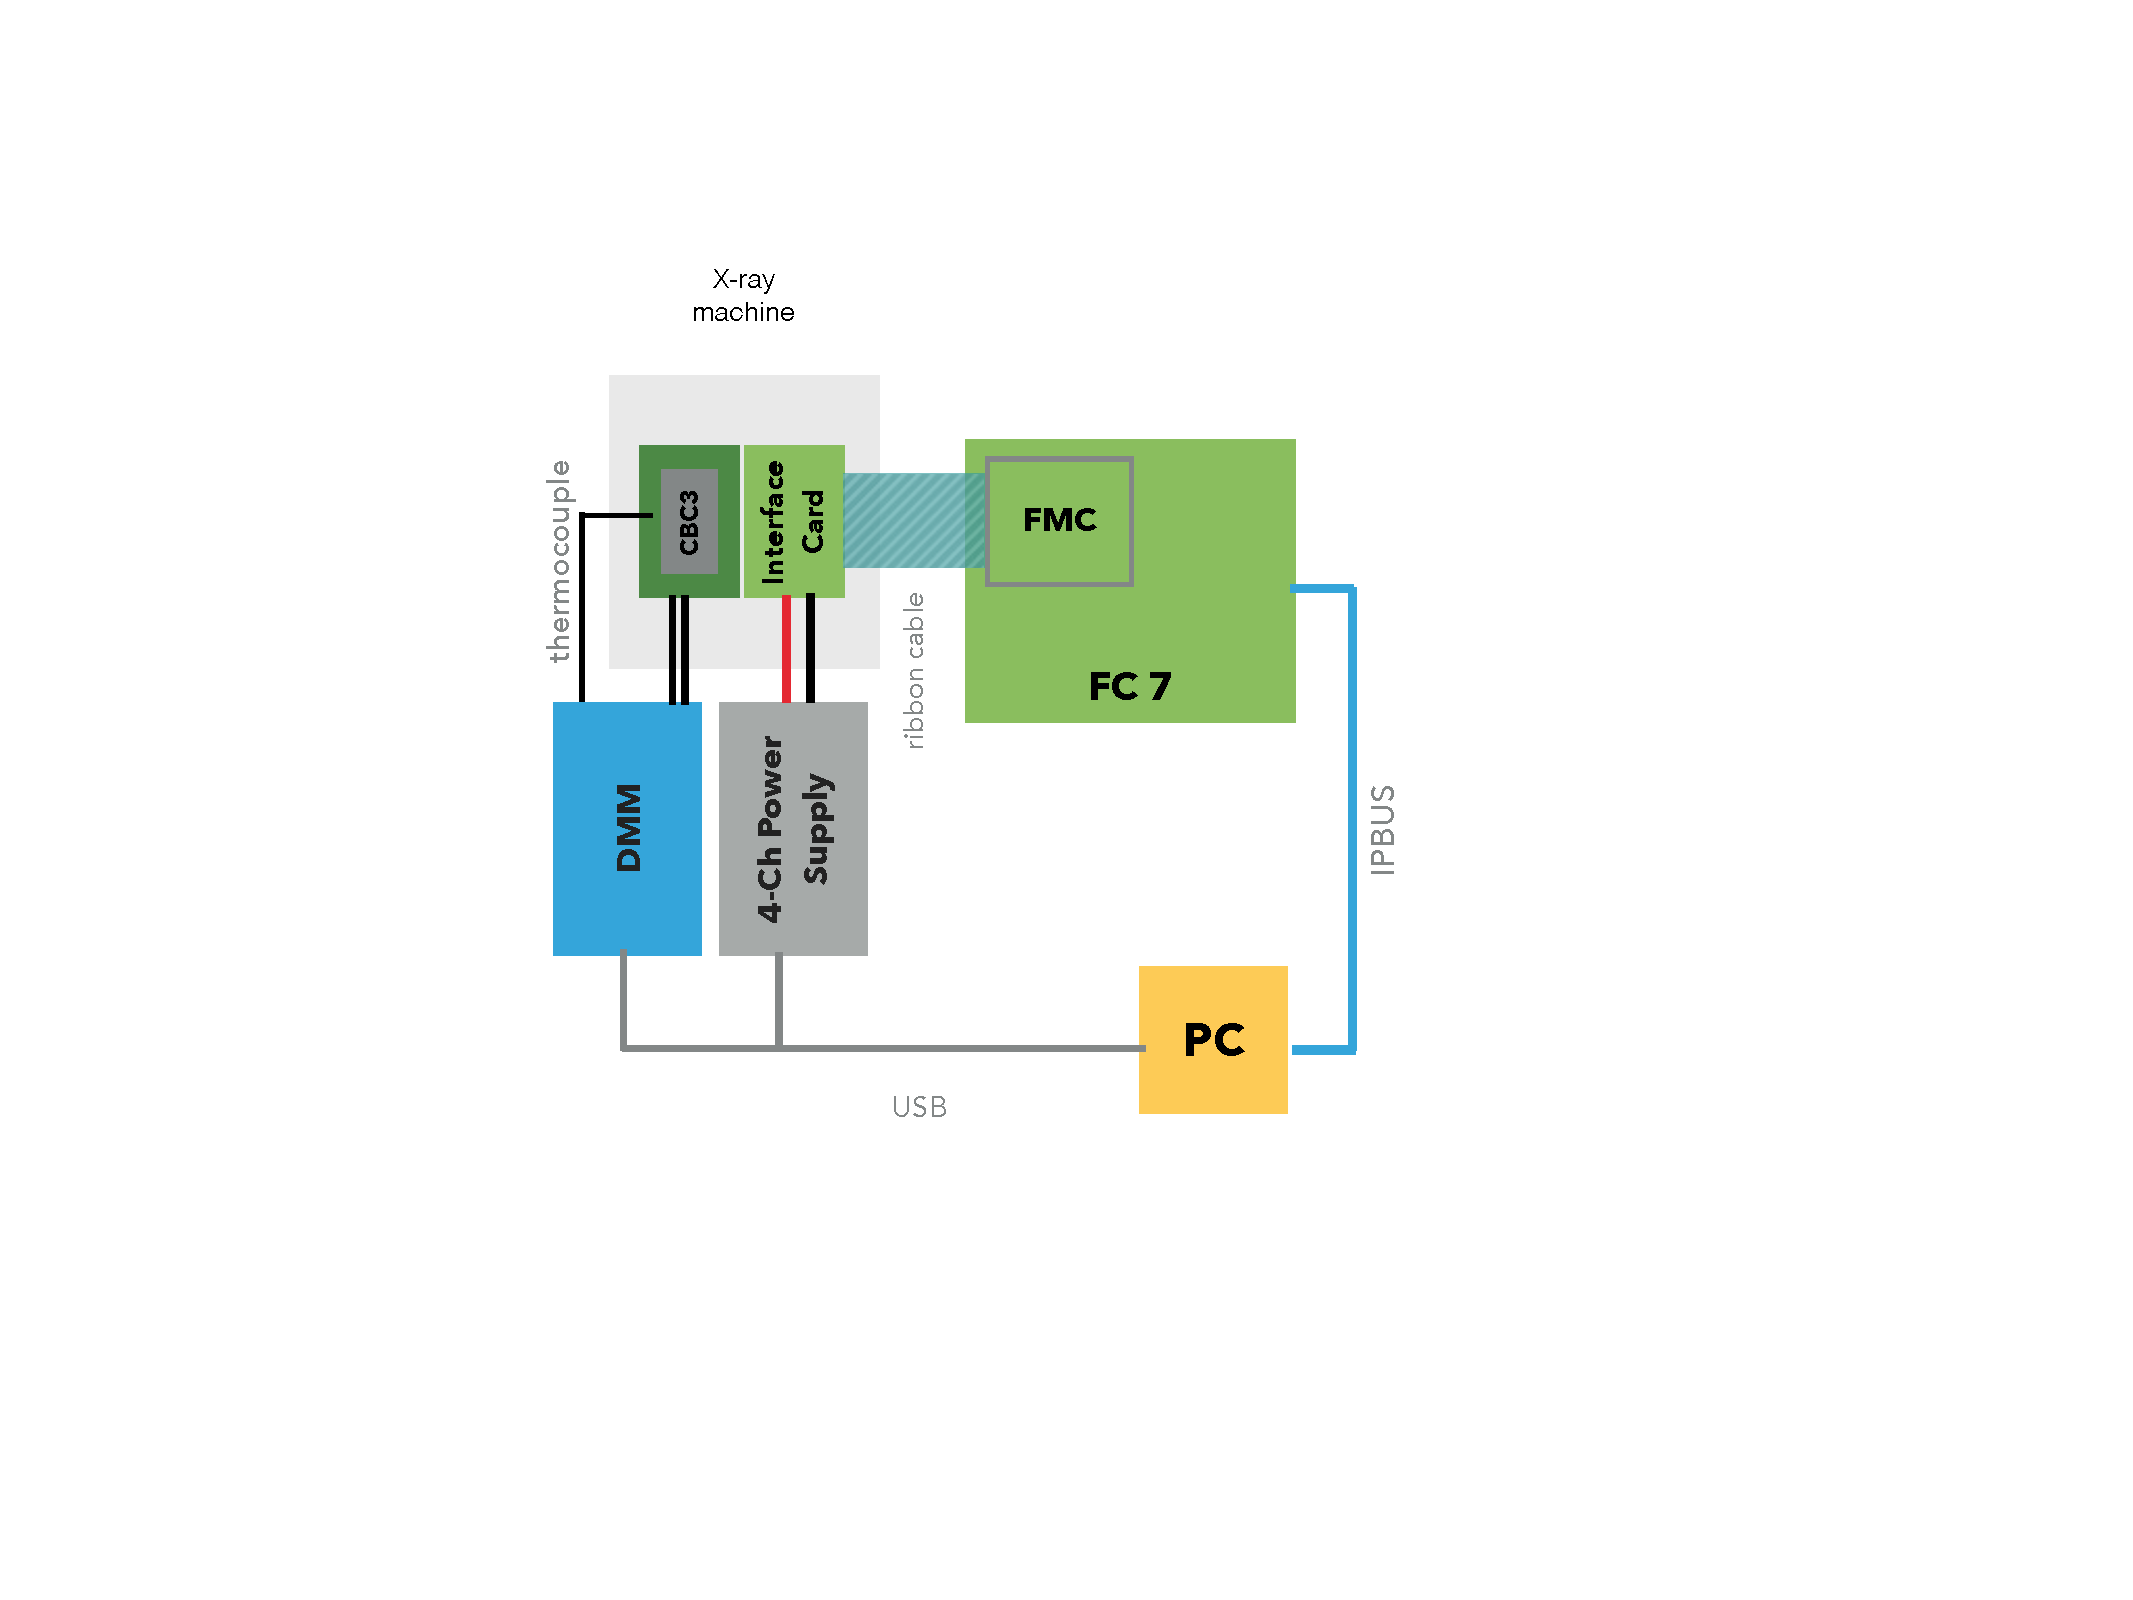
\includegraphics[width=0.8\linewidth]{Figures/SchematicSetup.pdf}
%   	\label{fig:daq}
%   }
%   \caption[Fit.]{DAQ system consisting of an FC7, a \textmu TCA Advanced Telecommunications Computing Architecture (ATCA) card and an interface card. A 1.5~m shielded ribbon cable was used to connect the interface card to the FC7 via a custom FPGA Mezanine Card.}
%   \label{fig:tst}
% \end{figure} 

% \begin{table}[htbp!]
% \begin{center}
%     \begin{tabular}{cccc}
%     \midrule
%         Voltage & Current & Distance & Dose Rate\\
%         $[$kV$]$ & $[$mA$]$ & $[$cm$]$ & $[$\kGyH$]$\\
%     \midrule
%     %\hline
%     $50$ & $40$ & $8$  & ${23.0\pm4.6}$\\
%     $50$ & $20$ & $8$  & ${11.6\pm2.3}$\\
%     $50$ & $10$ & $8$  & ${5.8\pm1.2}$\\
%     $50$ & $13$ & $18$ & ${2.4\pm0.5}$\\
%     $50$ & $10$ & $32$ & ${0.11\pm0.02}$\\
%     \midrule 
%   	\end{tabular}
% \caption{Dose rates and settings used for the CBC3 X-ray irradiation. The uncertainty on the dose rate is assumed to be 20\% of the value measured with the calibrated PIN diode. The dose was changed by adjusting either the vertical position of the CBC3 wrt the tube or by changing the tube's supply current.}
% \label{tab:calibration}
% \end{center}
% \end{table}
% don't really have space for this 
% \begin{figure}[htbp]
% \centering
% 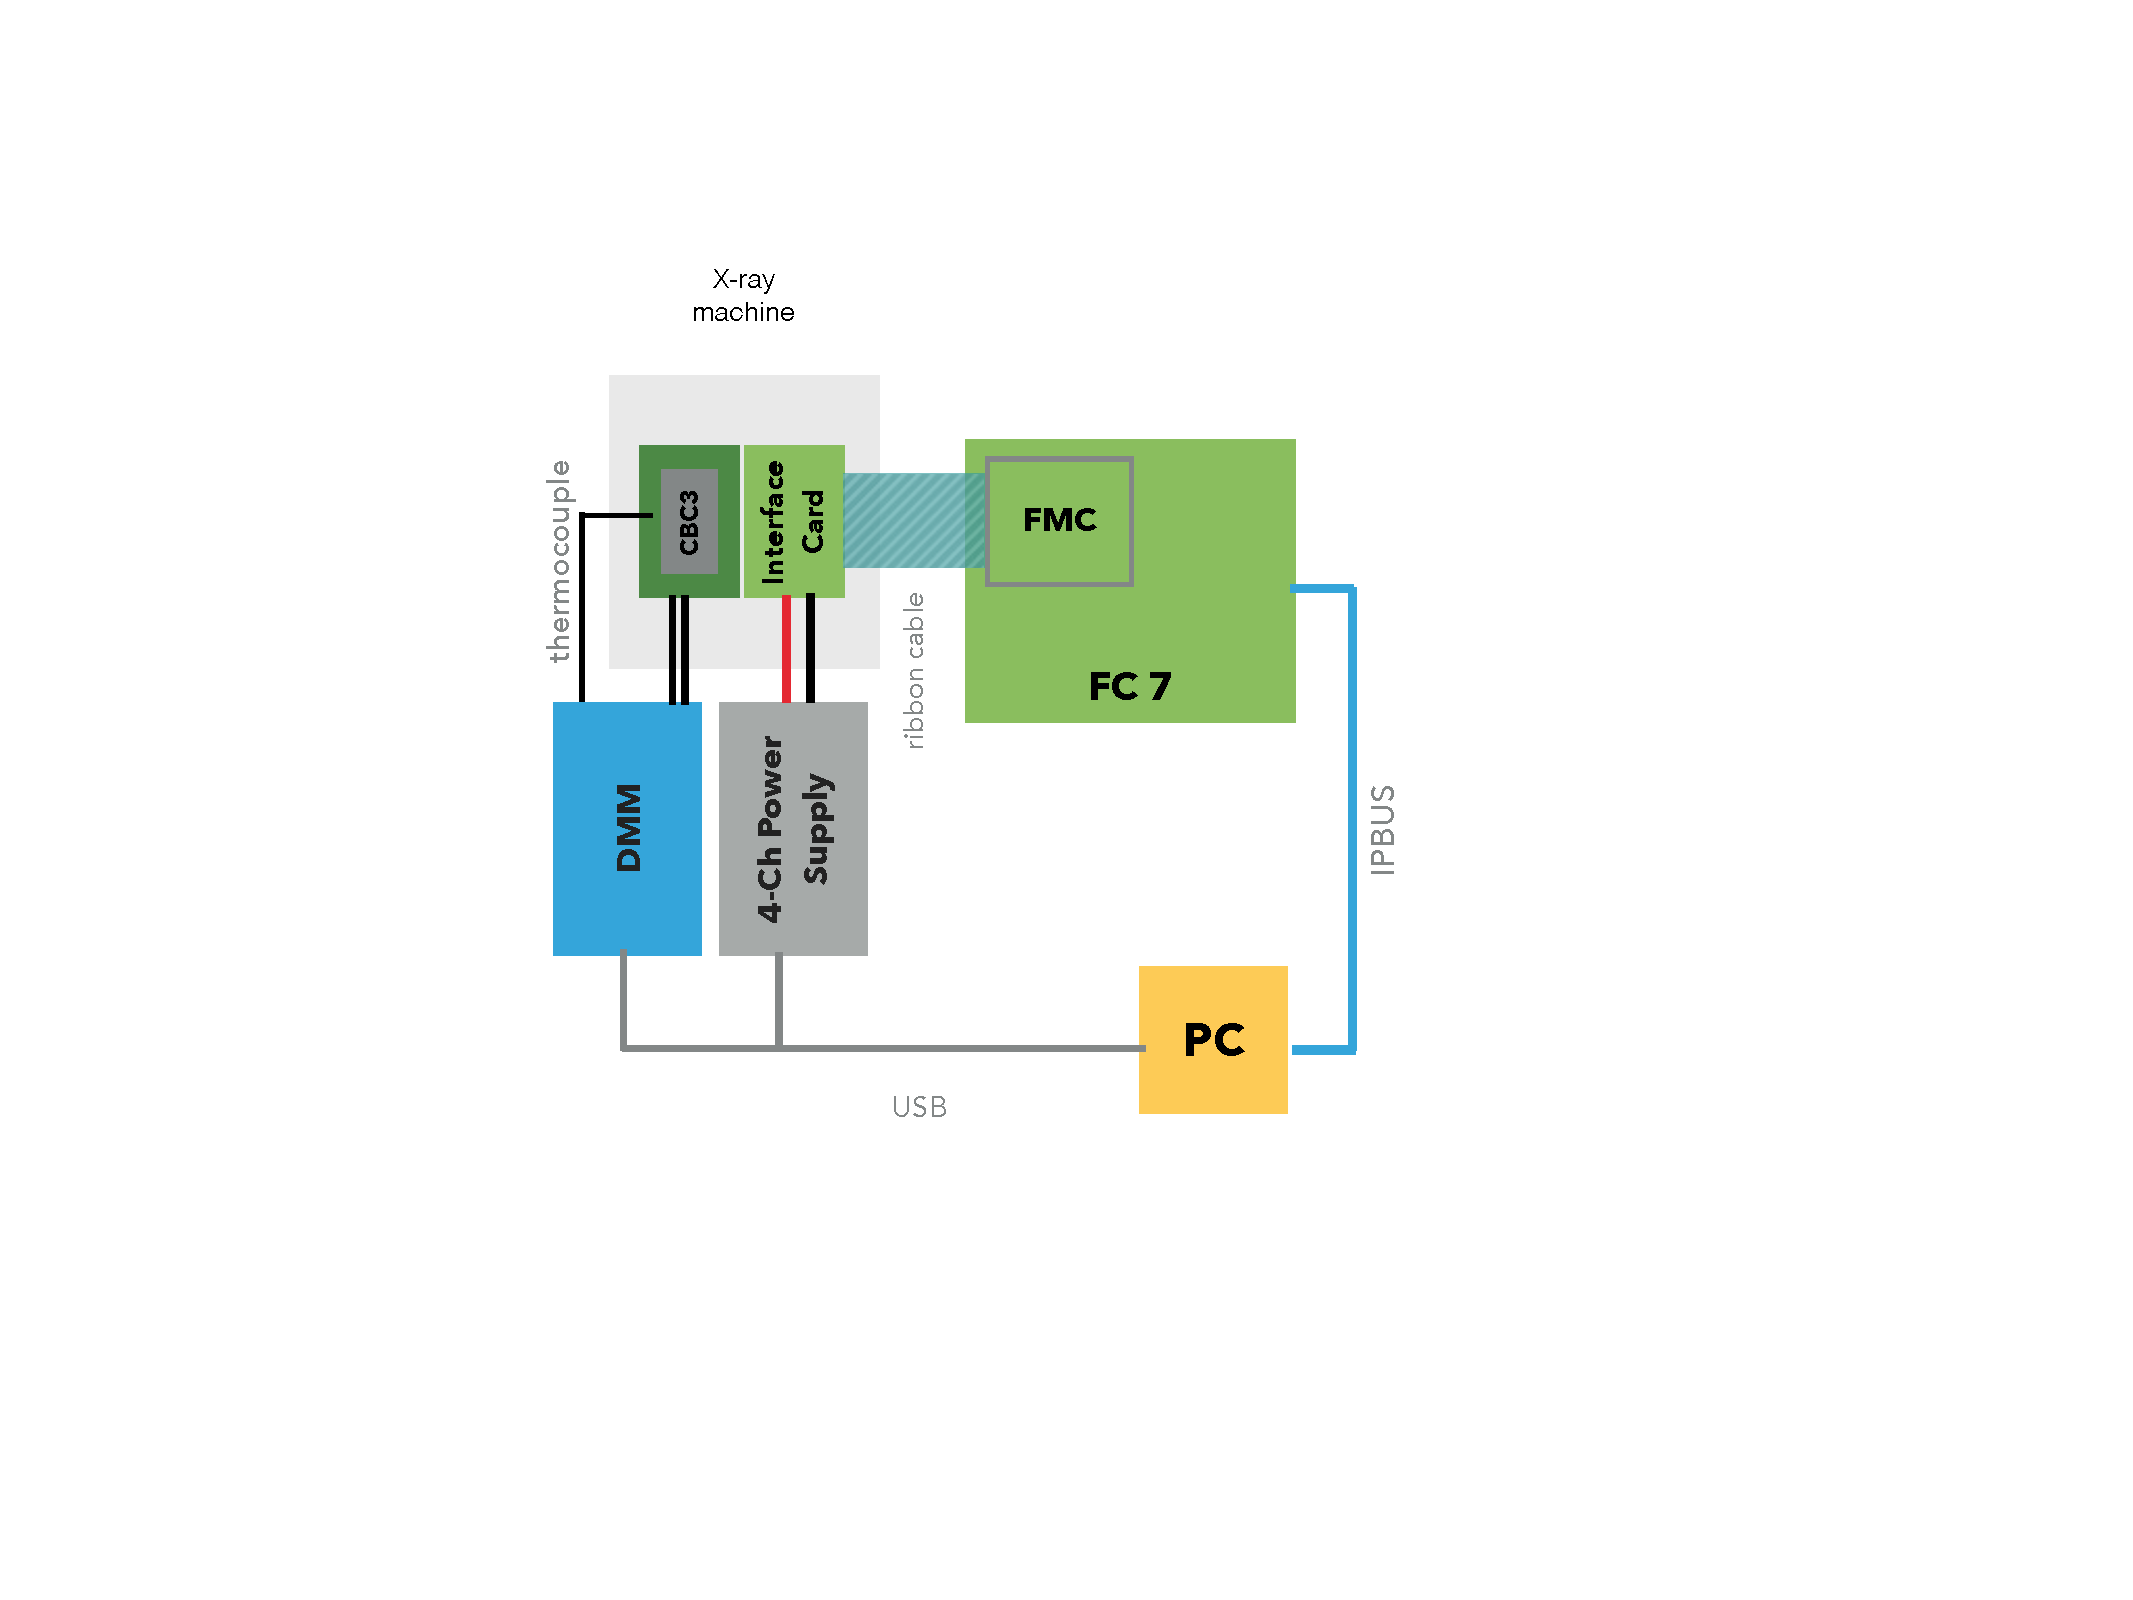
\includegraphics[width=0.65\linewidth]{Figures/SchematicSetup.pdf}
% \caption{DAQ system consisting of an FC7, a \textmu TCA Advanced Telecommunications Computing Architecture (ATCA) card and an interface card. A 1.5~m shielded ribbon cable was used to connect the interface card to the FC7 via a custom FPGA Mezanine Card.}
% \label{fig:daq}
% \end{figure}

To replicate realistic operating conditions, a prototype DAQ system  was used to provide the 320~MHz system clock, slow-control I2C commands, and clock-synchronous fast commands such as triggers and resets. The chips were wire-bonded to carrier boards plugged into an interface card, which provided the low voltage (1.25V) and level translation to interface to the DAQ. The interface card also provided monitoring of the digital and analogue currents, and the on-chip analogue bias signals.
% (via an on-chip 17:1 analogue multiplexer).

% A standard measurement cycle was repeated throughout the irradiation. The CBC3 was reconfigured at the start of each cycle. A tuning algorithm, designed to offset The individual channel offsets were then adjusted for a uniform response across the whole chip, with and without a test-pulse injected. This ensures that the global threshold is the same for all input channels and allows the measurement of the pedestal (the threshold corresponding to a noise occupancy of 50\%) and the noise per input channel. After calibration, the chip is triggered for a period of ten minutes at a high trigger rate with a channel occupancy of around 50\%, to ensure a high level of digital activity. The final part of the cycle involves stepping each analogue bias DAC setting through its full range, while holding the other DAC settings at their nominal values. The analogue biases are monitored externally with the multimeter, so this confirms the actual voltage for each DAC setting and checks if any of the control registers change their behavior in response to ionizing radiation. 
\section{Results}
\label{sec:Results}
\subsection{Current Consumption}
\label{subsec:DigiCurrent}
The current consumption of the digital and analogue circuits recorded during the irradiation of a CBC3 at 23\kGyH is shown in \Cref{fig:DigiCurrent}. 

\begin{figure}[!htbp]
\centering
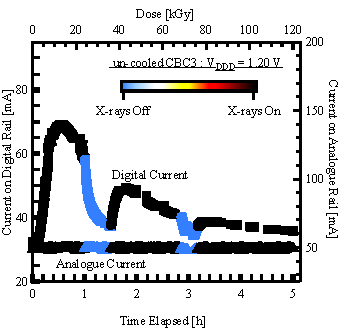
\includegraphics[width=0.8\linewidth]{Figures/DigiCurrent_CBC3_Uncooled.pdf}
\vspace*{-2mm}
\caption{Measured CBC3 digital (left axis) and analogue (right axis) currents during 
exposure to X-rays at the CERN X-ray irradiation facility. The color of the marker indicates the state of the X-ray machine during the measurement. 
%The cooling system was not active during this measurement.
}
\label{fig:DigiCurrent}
\end{figure}
% Needs a way to distinguish analogue from digital on the plot (S.S. too many points for the legend to be very useful... so added a label above each curve instead ) 
% Remove or explain arrows (S.S done!)
As with the previous version of the chip, a radiation-induced leakage current is observed for the CBC3.
%The radiation-induced leakage current observed in the previous version of the chip is still present in the CBC3.
The current consumed begins to increase after a few \kGy of dose and continues to increase up to a dose of approximately $15$\kGy beyond which it decreases exponentially towards the initial value.

% The dose rate and temperature of the CBC3 during the initial irradiation were not representative of those expected in the CMS OT. 
The initial irradiation was performed at a dose rate ${10^{4}}$ times higher than that expected for the 2S modules closest to the interaction point, with chips ${47}$\deg warmer than expected in the Phase-2 OT. Determining the magnitude of the current increase under realistic HL-LHC operating conditions therefore requires an understanding of the effect of temperature and dose rate on the radiation induced leakage current. This motivated the undertaking of a series of measurements at different temperatures and dose rates summarized in \Cref{fig:DigiCurrentSummary}.
%\cite{BragaThesis}
\begin{figure}[!htbp]
\centering
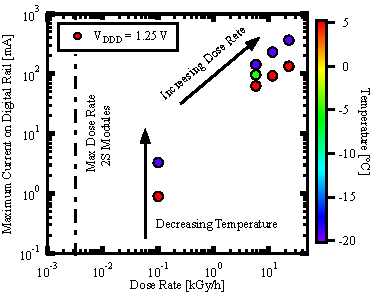
\includegraphics[width=0.8\linewidth]{Figures/DigiCurrent_CBC3_Summary_v2.pdf}
\vspace*{-5mm}
\caption{The (maximum) measured current consumption on the CBC3 digital rail as a function of dose rate. The color of the markers indicates the temperature at which the irradiation took place. All measurements used a bias voltage of $1.25$\,\volt.}
\label{fig:DigiCurrentSummary}
\end{figure}

The measured radiation induced increase in current rises for decreasing temperatures and increasing dose rates. The temperature of the CBCs when deployed in the Phase-2 OT will range from ${-17}$\deg to ${-9}$\deg; and the expected dose rate, indicated by a dashed line in \Cref{fig:DigiCurrentSummary}, is approximately $2$\% of the lowest dose rate reached in the X-ray irradiations. 

\subsection{Analogue Front-End Performance}
To verify robustness of the CBC3 analogue front-end against damage from ionizing radiation all parameters critical to its operation were monitored throughout. This included checking the behavior of  analogue bias registers, verification of  on-chip pipeline by measuring the response to the internal test pulse, and continuous monitoring of the pedestal and the noise.

% The CBC3 derives all analogue biases in the front end circuits using an on-chip bias generation circuit referenced by a radiation tolerant, PMOS transistor based, voltage reference bandgap. 
The two most important analogue biases are: the output of the band-gap reference ($V_{BG}$) circuit and the comparator threshold voltage ($V_{cth}$). $V_{BG}$ is the reference for all on-chip analogue biases, and $V_{cth}$ determines the global comparator threshold (shown in \Cref{fig:Architecture_AnalogueFE}). The resolution of $V_{th}$, provided by a 10 bit digital to analogue converter (DAC) with reference voltages provided by the analogue supply rail ($V_{DDA}$) and the on-chip ground (GND), is given by
\begin{equation}
V_{cth}\,\,[\frac{\mbox{\mV}}{\mbox{DAC units}}]=\frac{V_{DDA} - GND}{1024}=\frac{2V_{BG}-GND}{1024},
\label{eq:Vcth}
\end{equation}
where $V_{DDA}$ is twice $V_{BG}$. 
\begin{figure}[htbp]
\centering
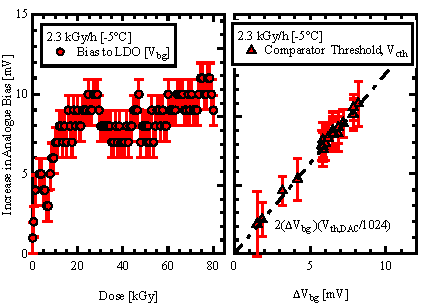
\includegraphics[width=0.9\linewidth]{Figures/Vbg_Irrad_v2.pdf}
\vspace*{-2mm}
\caption{$V_{BG}$ and $V_{cth}$ during irradiation; the comparator threshold corresponds to the output of the bias DAC at the nominal threshold setting of $\approx$580 DAC units.}
\label{fig:Vbg}
\end{figure}
%S.S. combined what was previously figures 6 and 7 into one plot - hopefully its not too squished in.

The evolution of the band-gap reference voltage during irradiation, and the corresponding change in $V_{cth}$, for a chip irradiated at $2.3$\kGyH and a temperature of -5\deg is shown in \Cref{fig:Vbg}. The measured $10$\mV\! increase (${O(2\%)}$) in the band-gap reference voltage of the chip is within the expected range (${\pm 12}$\mV\!) for the circuit used in the CBC3 \cite{Bandgap}; and the increase in threshold voltage is as expected from \Cref{eq:Vcth}. 

%I don't think I have enough space to show this 
% And then what about the noise? Complicated by the fact the cooling started before the start of the irradiation ...
% \begin{figure}[htbp]
% \centering
% 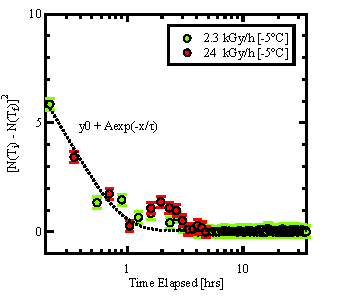
\includegraphics[width=0.8\linewidth]{Figures/Noise2_IncreaseIrrad.pdf}
% \caption{The size of reconstructed clusters in strips (635 $\mu$m
% strip pitch) for both readout coordinates of the central detector.}
% \label{fig:Noise2}
% \end{figure}
% Seems to be correlated with the increase in digital current. 
% \begin{figure}[htbp]
% \centering
% 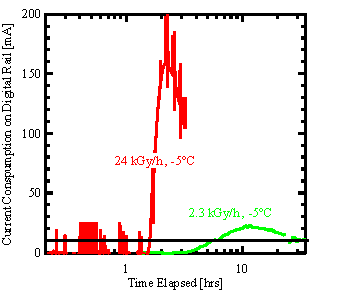
\includegraphics[width=0.8\linewidth]{Figures/Current_IncreaseIrrad.pdf}
% \caption{The size of reconstructed clusters in strips (635 $\mu$m
% strip pitch) for both readout coordinates of the central detector.}
% \label{fig:CurrentIncrease}
% \end{figure}

\begin{figure}[!htbp]
\centering
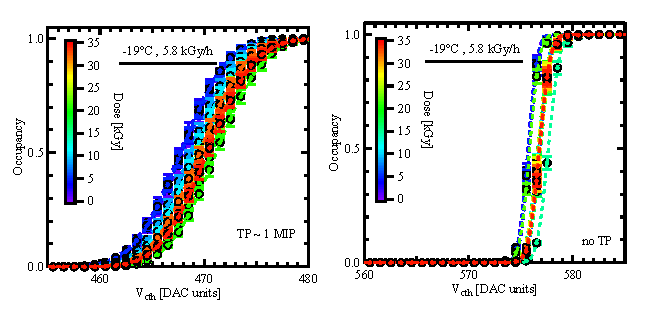
\includegraphics[width=1.1\linewidth]{Figures/Scurves_Chip4.pdf}
%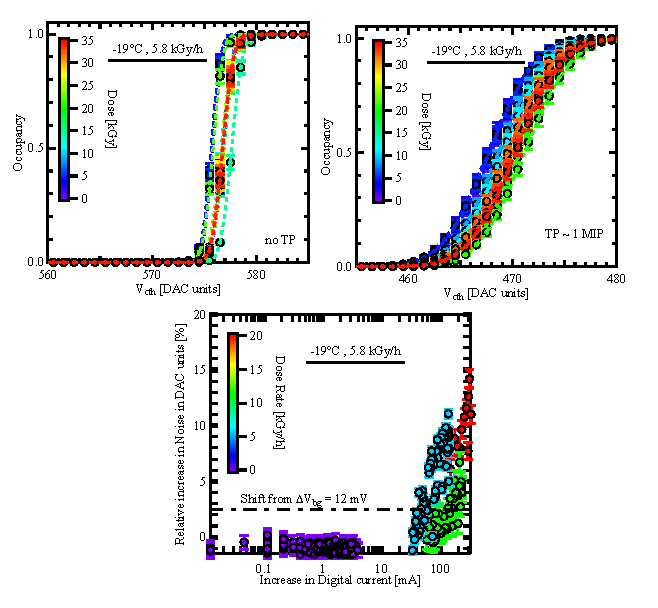
\includegraphics[width=0.99\linewidth]{Figures/test.pdf}
%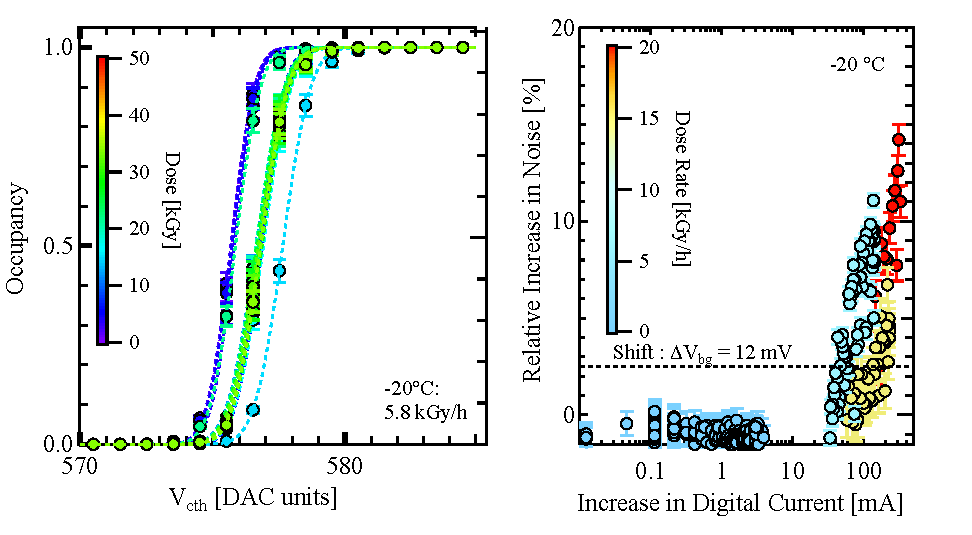
\includegraphics[width=1.1\linewidth]{Figures/NoiseIncrease_Summary_Chip4.pdf}
\vspace*{-10mm}
\caption{S-curves measured during the irradiation period: (left) using the on-chip test pulse to inject charge equivalent to 1 MIP, and (right) with no charge injected.The color of the markers indicates the dose received at the time of measurement, and the dashed lines the result of the fit using \Cref{eq:scurve}.}
\label{fig:Scurves}
\end{figure}

The noise and pedestal in a binary system such as the CBC3 must be inferred from an S-curve which shows the fraction of events in which a hit is detected as a function of the comparator threshold $V_{cth}$. Examples of S-curves collected during an irradiation are shown in \Cref{fig:Scurves}. Fitting the S-curve with a sigmoid of the form :
\begin{equation}
f(x, \mu, \sigma) =\frac{1}{2}[1 + \erf(\frac{x-\mu}{\sqrt{2}\sigma}) ],
\label{eq:scurve}
\end{equation}
returns the  pedestal (\textmu) and noise ($\sigma$). S-curves were also used to test the response of the CBC3 to the internal test pulse, by using the on-chip test pulse to inject charge into all 254 input channels on the CBC3. 
%missing \cite{BragaThesis}
%can be extracted directly from the S-curves by fitting them with a sigmoid of the form where \textmu and $\sigma$ correspond to the pedestal the noise respectively.  
As \Cref{fig:Scurves} shows, the CBC3 remains responsive to the test pulse in the presence of a large leakage current (${\approx 200}$\mA). This indicates that enclosed pipeline transistors in the CBC3 mitigated effects observed in the previous version. The noise and pedestals measured for different dose rates are shown in \Cref{fig:noisePede}. It shows that the increase in noise observed during irradiation at high dose rate is correlated with the radiation induced leakage current; no change in noise is observed as long as the increase in current remains below ${10}$\mA.


\begin{figure}[!htbp]
\centering
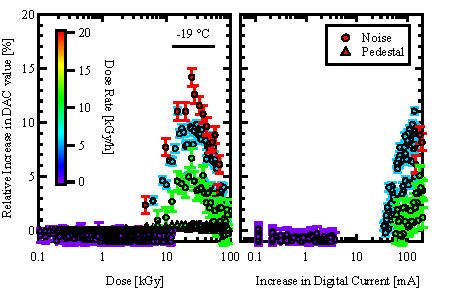
\includegraphics[width=0.9\linewidth]{Figures/NoisePede_Summary.pdf}
%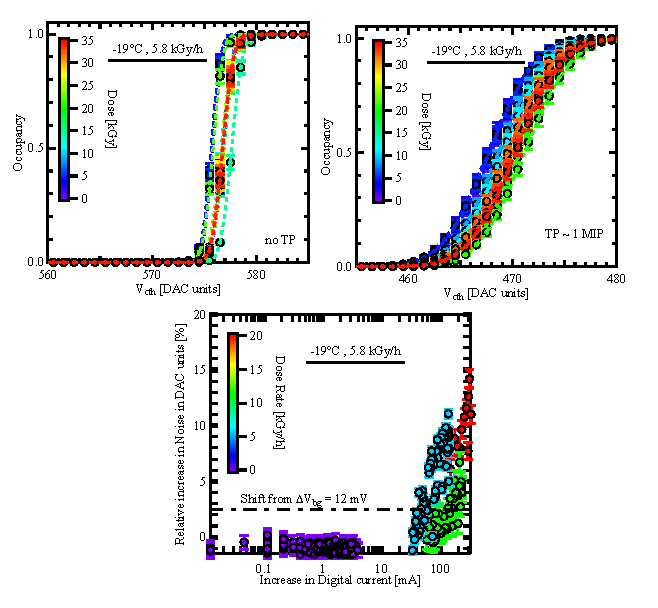
\includegraphics[width=0.99\linewidth]{Figures/test.pdf}
%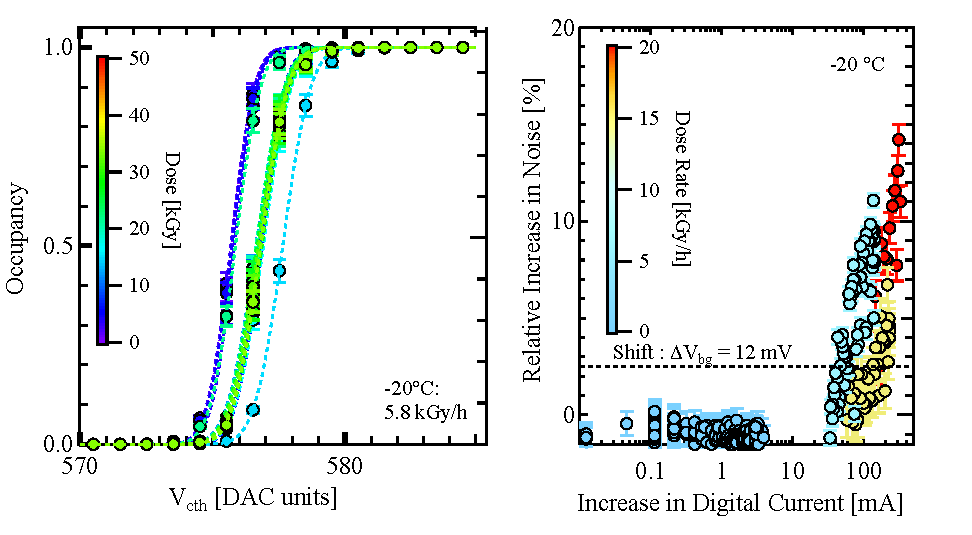
\includegraphics[width=1.1\linewidth]{Figures/NoiseIncrease_Summary_Chip4.pdf}
\vspace*{-2mm}
\caption{Noise and pedestal as a function of dose(left) , and correlation between noise and increase in digital current (right).The color of the markers indicates the dose rate at which the irradiation took place.}
\label{fig:noisePede}
\end{figure}

%Summarize performance ... and motivate radiation damage model 


%$-19$\deg can be used to place an upper limit on the maximum current expected in the CBCs in the Phase-2 OT conditions
\section{Radiation Damage Model}
The data collected with the CERN X-ray source  (\Cref{fig:DigiCurrentSummary}) was used to develop a model to predict an upper limit for the expected current increase in a 2S module under HL-LHC operating conditions. The model extends that proposed by Backhaus et al \cite{BackhausFeI4}, where the leakage current is attributed to the creation of leakage paths between source and drain via the inversion layer. The leakage paths are described as parasitic transistors, each with a transfer characteristic given by 
%created in the silicon along the \interface interface of the oxide
\begin{eqnarray}
I_D \approx 0 \,\,\,\,\,: \Neff < \Nthr \\
I_D \approx K_0~(\Neff - \Nthr)^2 \,\,\,\,\,: \Neff \ge \Nthr ,
\label{eq:TransferCharacteristic_ParasiticTransistors}
\end{eqnarray}
where $\Neff$ is the effective number of charges located in the inversion layer created by the build-up of positive charge in the oxide, $\Nthr$ is the threshold number of charges required to activate the transistor, and ${K_0}$ is a proportionality constant.
\begin{figure}[htbp]
\centering
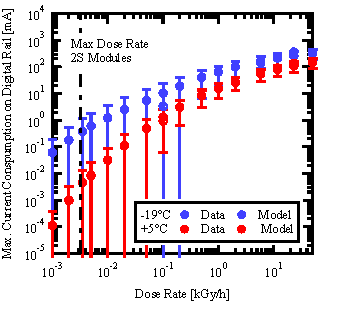
\includegraphics[width=0.8\linewidth]{Figures/ModelPrediction_CurrentConsumption.pdf}
\vspace*{-5mm}
\caption{The size of reconstructed clusters in strips (635 $\mu$m
strip pitch) for both readout coordinates of the central detector.}
\label{fig:ModelComparison_CurrentIncrease}
\end{figure}

The effective number of charges in the transistor can be expressed as
\begin{equation}
\Neff = \Not - \Nit. 
\label{eq:Neff}
\end{equation}
where ${\Not}$ and ${\Nit}$ are the positive trapped charge and interface traps created \cite{BarnabyTIDeffects} when electron-hole pairs (ehps) generated by ionization interact with existing defects and impurities in the oxide. Holes that survive initial prompt recombination may be trapped by deep traps as they move throughout the oxide; while those not trapped by defect sites are free to interact with hydrogen-containing defects ($D^{'}H$) introduced in the oxide during its growth. The simplest of these interactions releases a proton ($H^+$) from the defect site. Interface traps are created when a proton produced by such a reaction reaches the \interface interface and removes a hydrogen molecule ($H_2$) from a dangling bond (${SiH}$); creating an interface trap.
% Trapped holes, i.e. trapped positive charge $\Not$, have a finite probability of escaping from these traps depending on the energy level(s) of the traps and the temperature of the device during irradiation. 

The rate of creation of trapped positive charge in the oxide can therefore be given by
\begin{equation}
\dot N_{\mbox{\tiny{OT}}} = f_{\mbox{\tiny{OT}}}k_0\,\dot D\,(\NotMax - \Not)- \Rot\,\Not ,
\label{eq:Not_TrappingRate}
\end{equation}
where $f_{\mbox{\tiny{OT}}}$ is a deep trap's hole trapping probability, ${k_0}$ is a constant proportional to the introduction rate of holes in the oxide, $\Rot$ is the de-trapping rate of holes, $\NotMax$ is the maximum number of deep trapping sites in the oxide, and ${\dot D}$ is the dose rate. In addition, the rate of proton release can expressed as 
\begin{equation}
\dot p = f_p\,(k_0\,\dot D - \dNot)\,(N_p - p),
\label{eq:Proton_ReleaseRate}
\end{equation}
where ${f_p}$ is a hydrogen-containing defect's proton trapping a hole, ${(k_0\,\dot D - \dNot)}$ describes the number of holes available to participate in this process, and ${N_p}$ is the maximum number of available hydrogen-containing defects in the oxide. Finally, the rate of interface trap creation can be modeled by 
\begin{equation}
\dot N_{\mbox{\tiny{IT}}} = f_I\,(N_{\mbox{\tiny{SiH}}} - N_{\mbox{\tiny{IT}}}) \dot p, 
\label{eq:Nit_TrappingRate_0}
\end{equation}
 where ${f_I}$ is the probability that an available dangling bond captures the free proton, and $\NitMax$ is the number of hydrogen-passivated dangling bonds present in the un-irradiated oxide. An analytical description for the number of fixed positive charges $\Not$ and interface traps $\Nit$ created during an irradiation can be found by solving the system of coupled differential equations described by ~\Cref{eq:Not_TrappingRate,eq:Proton_ReleaseRate,eq:Nit_TrappingRate_0}. The solution for the case where the irradiation starts at ${t=0}$ is given by
\begin{eqnarray}
\Nit = \NitMax\,[1 - e^{- p(t)}] \\ 
\Not = \NotMax\,\frac{\Fot k_0 \dot D}{\Fot k_0 \dot D + \Rot}\,[1 - e^{-(\Fot k_0 \dot D + \Rot)t}] \\
p(t) = f_I\,N_p[ 1 - e^{-f_p k_0\,\dot D\,t + f_p\,\Not(t)} ].
\label{eq:Solution_DifferentialEquations}
\end{eqnarray}

A simultaneous fit of the parametrized damage model to the data collected for each set of four chips irradiated at $-19$\deg and $5$\deg was used to extract the dose-rate dependence of the model parameters. The predicted current increase at the expected HL-LHC dose rate and $-19$\deg, shown in \Cref{fig:ModelComparison_CurrentIncrease}, is believed to be a conservative upper limit on the current increase expected in 2S modules due to radiation induced leakage in the CBC3s. 

%(e.g. oxygen vacancies in the oxide bulk and/or hydrogen passivated dangling  bonds at the \interface interface).
% and the total (digital) leakage current of the CBC3 when exposed to ionizing radiation can be written as 
% \begin{equation}
% \Ileak = \IpreIrrad + K~(\Not - \Nit - \Nthr)^2 \,\,\mbox{for}\,\, \Neff \ge \Nthr , 
% \label{eq:LeakageCurrent_CBC3}
% \end{equation} 
% where $K$ is a new proportionality constant that takes into account that the total leakage current measured in the CBC3 is the sum of the additional current flowing through the many thousands of transistors that make up the digital logic of the CBC3.


% In the case of NMOS transistors (of the type used in the CBC3) the build-up of positive charge in the oxide results in positive charge ($\Not$) build-up, whilst the creation of interface traps ($\Nit$) at the \interface interface results in a negative space charge. Therefore the effective number of charges in the transistor can be expressed as
% \begin{equation}
% \Neff = \Not - \Nit. 
% \label{eq:Neff}
% \end{equation}
% and the total (digital) leakage current of the CBC3 when exposed to ionizing radiation can be written as 
% \begin{equation}
% \Ileak = \IpreIrrad + K~(\Not - \Nit - \Nthr)^2 \,\,\mbox{for}\,\, \Neff \ge \Nthr , 
% \label{eq:LeakageCurrent_CBC3}
% \end{equation} 
% where $K$ is a new proportionality constant that takes into account that the total leakage current measured in the CBC3 is the sum of the additional current flowing through the many thousands of transistors that make up the digital logic of the CBC3.

% Positive trapped charge and interface traps at the \interface interface are created in a CMOS circuit exposed to ionizing radiation when electron-hole pairs (ehps) generated by the ionizing radiation interact with existing defects and impurities (e.g. oxygen vacancies in the oxide bulk and/or hydrogen passivated dangling  bonds at the \interface interface).
%which is dependent on the energy level(s) of the deep traps located in the oxide and the temperature at which the irradiation takes place.

%\cite{BarnabyTIDeffects}
% Holes not trapped by defect sites are free to interact with hydrogen containing defects ($D^{'}H$) introduced in the oxide during its growth. The simplest of these interactions acts to release a proton ($H^+$) from the defect site with a rate of proton release given by
% \begin{equation}
% \dot p = f_p\,(k_0\,\dot D - \dNot)\,(N_p - p),
% \label{eq:Proton_ReleaseRate}
% \end{equation}
% where ${f_p}$ is a hydrogen containing defect's proton trapping a hole, ${(k_0\,\dot D - \dNot)}$ describes the number of holes available to participate in this process, and ${N_p}$ is the maximum number of available hydrogen containing defects in the oxide. Interface traps are created when a proton produced by such a reaction reaches the \interface interface. The rate of interface trap creation can therefore be written as
% \begin{equation}
% \dot N_{\mbox{\tiny{IT}}} = f_I\,(N_{\mbox{\tiny{SiH}}} - N_{\mbox{\tiny{IT}}}) \dot p, 
% \label{eq:Nit_TrappingRate_0}
% \end{equation}
%  where ${f_I}$ is the probability that an available dangling bond captures the free proton, and $\NitMax$ is the number of hydrogen passivated dangling bonds present in the un-irradiated oxide.

% An analytical description for the number of fixed positive charges $\Not$ and interface traps $\Nit$ created during an irradiation can be found by solving the system of coupled differential equations described by ~\Cref{eq:Not_TrappingRate,eq:Proton_ReleaseRate,eq:Nit_TrappingRate_0}. The solution for the case where the irradiation starts at ${t=0}$ is given by
% \begin{eqnarray}
% \Nit = \NitMax\,[1 - e^{- p(t)}] \\ 
% \Not = \NotMax\,\frac{\Fot k_0 \dot D}{\Fot k_0 \dot D + \Rot}\,[1 - e^{-(\Fot k_0 \dot D + \Rot)t}] \\
% p(t) = f_I\,N_p[ 1 - e^{-f_p k_0\,\dot D\,t + f_p\,\Not(t)} ].
% \label{eq:Solution_DifferentialEquations}
% \end{eqnarray}
% This can then be used to fit the increase in the leakage current ${\Ileak - \IpreIrrad}$ measured at different dose rates and temperatures with the CERN X-ray source. The dose rate dependence of the model parameters in this model are used to predict the expected current increase at dose rates beyond those measured here, as shown in \Cref{fig:ModelComparison_CurrentIncrease}.


% The damage model developed by Backhaus et. al attributes the leakage current increase of linear NMOS transistors to the creation of leakage paths between source and drain via the inversion layer created in the silicon along the \interface interface of the STI. 
% \begin{figure}[!htbp]
%  \centering
%   \subfloat[][Pre-irradiation.]
%   {
%     \includegraphics[width=0.25\columnwidth]{./Fig/NMOS_PreIrrad.eps}
%     \label{fig:NMOS_preIrrad}
%   }
%   \quad
%   \subfloat[][Post-irradiation (gate removed).]
%   {
%     \includegraphics[width=0.25\columnwidth]{./Fig/NMOS_Irrad.eps}
%     \label{fig:NMOS_Irrad}
%   }
%  \caption[Linear NMOS transistor before and after exposure to ionizing radiation.]{Top views of a linear NMOS transistor before (left) and after (right) exposure to ionizing radiation. The fixed positive charge built up in the STI and the corresponding inversion layer created in the channel of the transistor are also shown.}
%  \label{fig:NMOS}
% \end{figure} 
% The leakage current paths are described in \cite{BackhausFeI4} as parasitic with a transfer characteristic 
% \begin{eqnarray}
% I_D \approx 0 \,\,\,\,\,: \Neff < \Nthr \\
% I_D \approx K_0~(\Neff - \Nthr)^2 \,\,\,\,\,: \Neff \ge \Nthr ,
% \label{eq:TransferCharacteristic_ParasiticTransistors}
% \end{eqnarray}
% where $\Neff$ is the effective number of charges located in the inversion layer created in the silicon by the build-up of positive charge in the STI, $\Nthr$ is the threshold number of charges required to activate the transistor, and ${K_0}$ is a proportionality constant containing the widths, lengths, oxide capacitance and the mobility of the minority charge carriers in the channel of the transistor. In the case of NMOS transistors (of the type used in the CBC3) the build-up of positive charge in the STI results in positive charge, whilst the creation of interface traps at the \interface interface results in a negative space charge. Therefore the effective number of charges in the transistor can be expressed as
% \begin{equation}
% \Neff = \Not - \Nit. 
% \label{eq:Neff}
% \end{equation}

% Therefore the total (digital) leakage current of the CBC3 when exposed to ionizing radiation can be written as 
% \begin{equation}
% \Ileak = \IpreIrrad + K~(\Not - \Nit - \Nthr)^2 \,\,\mbox{for}\,\, \Neff \ge \Nthr , 
% \label{eq:LeakageCurrent_CBC3}
% \end{equation} 
% where $K$ is a new proportionality constant that takes into account that the total leakage current measured in the CBC3 is the sum of the additional current flowing through the many thousands of transistors that make up the digital logic of the CBC3 and ${\Not,\Nit}$ are the solutions to the rate equations derived for the build-up of positive fixed charge and interface traps derived in \Cref{subsec:Not,subsec:Nit}.

% %re-phrase this... needs thinking (want to say why this effect is present only in NMOS)
% % The space charge in the STI is always positive and therefore in PMOS transistors this transistor channel is closed by the radiation induced space charge. Thus the leakage current increase is only observed in NMOS transistors.

% Finding an analytical description for the number of fixed positive charges $\Not$ and interface traps $\Nit$ created during an irradiation requires solving the system of coupled differential equations described by ~\Cref{eq:Not_TrappingRate,eq:Proton_ReleaseRate,eq:Nit_TrappingRate_0}. The solution for the case where the irradiation starts at ${t=0}$ is given by
% \begin{eqnarray}
% \Nit = \NitMax\,[1 - e^{- p(t)}] \\ 
% \Not = \NotMax\,\frac{\Fot k_0 \dot D}{\Fot k_0 \dot D + \Rot}\,[1 - e^{-(\Fot k_0 \dot D + \Rot)t}] \\
% p(t) = f_I\,N_p[ 1 - e^{-f_p k_0\,\dot D\,t + f_p\,\Not(t)} ],
% \label{eq:Solution_DifferentialEquations}
% \end{eqnarray}
% (the details of the solution are provided in the appendix). \Cref{eq:LeakageCurrent_CBC3,eq:Solution_DifferentialEquations} can then be used to fit the increase in the leakage current ${\Ileak - \IpreIrrad}$ measured at different dose rates and temperatures with the CERN X-ray source. If the fit can also be used to establish the dose rate dependence of the model parameters then this model can be used to predict the expected current increase at dose rates beyond those measured here. The following section describes how this was achieved using the results from the X-ray irradiation of the CBC3s at temperatures of ${-19}$\deg/5\deg and a bias voltage of $1.25\,$\volt. 

% % \begin{figure}[htbp]
% % \centering
% % 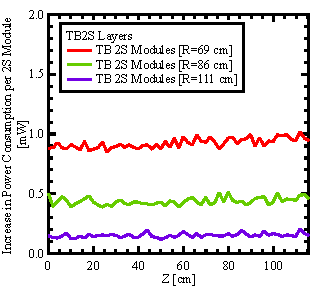
\includegraphics[width=0.8\linewidth]{Figures/ModelPrediction_PowerConsumption.pdf}
% % \caption{The size of reconstructed clusters in strips (635 $\mu$m
% % strip pitch) for both readout coordinates of the central detector.}
% % \label{fig:ModelPredictionPower}
% % \end{figure}


\section{Stub Finding in the CBC3}
The CBC3 is the first version of the 2S module read-out ASIC to include the full logic circuitry required for stub finding. A 2S module prototype, constructed with two sensors separated by ${1.8}$\mm and a double-sided rigid hybrid with two bump-bonded CBC3 chips, was used to test the logic using the 120 GeV proton beam at the Fermilab Test Beam Facility. \Cref{fig:stubs} shows the stub-finding efficiency for different correlation windows : a programmable on-chip register which defines the maximum distance (in strips) between clusters on a valid stub. The measurement shows that the stub is high (${>95\%}$) and that the cut-off is in agreement with that expected for the given sensor strip pitch and spacing.

% This exploits the relationship between a proton's angle of incidence ($\theta$) on the module and the longitudinal seperation (${\delta x}$) between the corresponding hits in the two sensors ; on a module at radius $R$ is exploited to emulate the effect of a $3.8$\,\tesla\, magnetic field on charged particles  
% \begin{equation}
% p_T = \frac{0.57R}{\sin(\theta)}\approx0.57R\sqrt{1 + (\frac{d}{\Delta{x}})^2}
% \end{equation}

\begin{figure}[!htbp]
\centering
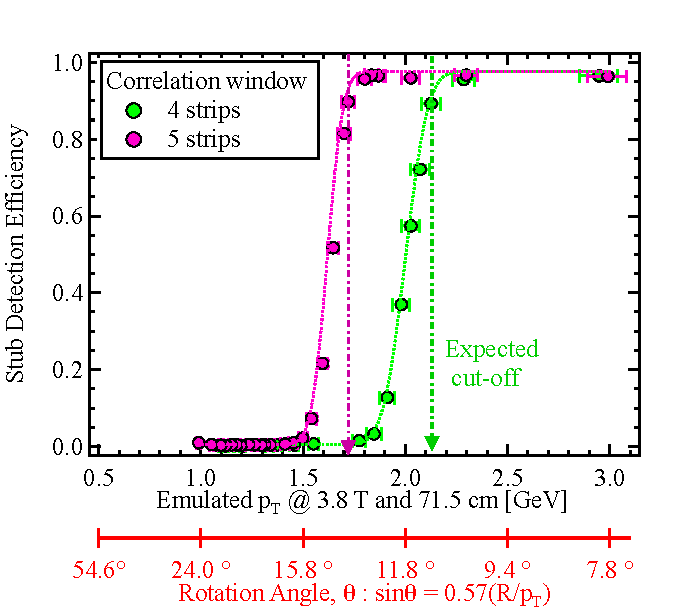
\includegraphics[width=0.9\linewidth]{Figures/StubScan.pdf}
\vspace*{-2mm}
\caption{Stub detection efficiency as a function of emulated transverse momemtum ${p_T}$; the expected ${p_T}$ cut-off estimated from the strip pitch (${90}$\microns) and the sensor spacing ${1.8}$\mm is also shown. The prototype was rotated with respect to the beam-axis to mimic the effect of charged particles bending in a magnetic field at a radius $R$ of ${71.5}$\cm.}
\label{fig:stubs}
\end{figure}

\section{Conclusion}
An extensive irradiation campaign at CERN and a test beam at the Fermilab test beam facility have verified the functionality of the CBC3, the final prototype ASIC for the CMS OT 2S modules. The measurements have shown the CBC3 to be capable of withstanding HL-LHC radiation levels, and have demonstrated the CBC3's ability to identify high ${p_T}$ tracks with high efficiency. 

A radiation damage model has been developed, using data collected during the irradiations, to predict the expected increase in power consumption for HL-LHC operation. The maximum expected current increase in the CBCs would increase power consumption of a 2S module by approximately 20 mW (there are ${\times16}$ CBCs per 2S module ) which corresponds to a less than ${1}$\% increase in the total power consumption of a module.


%\section*{Acknowledgments}
%% bibliography
\bibliographystyle{IEEEtran}
\bibliography{Bibliography_SA}
% \begin{thebibliography}{10}
% \expandafter\ifx\csname url\endcsname\relax
%   \def\url#1{\texttt{#1}}\fi
% \expandafter\ifx\csname urlprefix\endcsname\relax\def\urlprefix{URL }\fi


% \bibitem{Sauli:1997qp}
% F.~Sauli, {GEM}: A new concept for electron amplification in gas detectors,
%   Nucl. Instrum. Meth. A386 (1997) 531--534.

% \bibitem{Altunbas:2002ds}
% M.~C. Altunbas, et~al., Construction, test and commissioning of the
%   triple-{GEM} tracking detector for {COMPASS}, Nucl. Instrum. Meth. A490
%   (2002) 177--203.

% \bibitem{Simon:2007sk}
% F.~Simon, et~al., {Development of Tracking Detectors with industrially produced
%   GEM Foils}, IEEE Trans. Nucl. Sci. 54 (2007) 2646--2652.

% \bibitem{Simon:2007fz}
% F.~Simon, The {STAR} tracking upgrade, arXiv:0710.0172 [physics.ins-det].

% \bibitem{Ackermann:2002ad}
% K.~H. Ackermann, et~al., {STAR} detector overview, Nucl. Instrum. Meth. A499
%   (2003) 624--632.

% \bibitem{Allgower:2002zy}
% C.~E. Allgower, et~al., The {STAR} endcap electromagnetic calorimeter, Nucl.
%   Instrum. Meth. A499 (2003) 740--750.

% \end{thebibliography}
\end{document}